\documentclass[11pt]{article}
\usepackage[margin=1in]{geometry}
\usepackage{graphicx}
\usepackage{booktabs}
\usepackage{siunitx}
\usepackage{caption}
\captionsetup{font=small}
\sisetup{round-mode=places,round-precision=1}

\title{Analysis of EASY-Based Scheduling Heuristics}
\author{SPARS Scheduler Experiments}
\date{\today}

\begin{document}
\maketitle

\section{Overview}
All experiments use the workload defined in \texttt{Tugas\_HandsOn/workload.json}, comprising 200 jobs with staggered submission times. We compared two custom heuristics that extend the base EASY scheduler:
\begin{itemize}
  \item \textbf{EASYBalanced} (\texttt{SPARS/Simulator/Algo/easy\_balanced.py}) inherits the EASY backfilling loop but only wakes sleeping nodes after a wait threshold is exceeded and no imminent release of active nodes is predicted. Sleeping machines therefore stay offline longer, reducing energy draw at the cost of longer queues when the cluster is under tight power management.
  \item \textbf{EASYAdaptive} (\texttt{SPARS/Simulator/Algo/easy\_adaptive.py}) starts from the balanced heuristic but lowers the wake threshold dynamically based on queue length and shortfall size. Small deficits trigger immediate wake-ups, while large deficits still require convincing signals (long waits or distant releases). This trades additional energy for shorter waiting time when the system is busy.
\end{itemize}
Both algorithms retain EASY backfilling~\cite{easy} to fill idle gaps after the head job is planned, so the latency differences stem solely from the wake-up policy.

\section{Experimental Setup}
For each algorithm we swept timeout values from \SI{300}{\second} to \SI{3600}{\second} in \SI{300}{\second} increments. The timeout governs the node power-management policy enforced by the simulator. After each run we recorded:
\begin{align}
  \bar{W} &= \frac{1}{N} \sum_{i=1}^{N} \left( t^{\text{start}}_{i} - t^{\text{sub}}_{i} \right), \\
  E_{\mathrm{waste}} &= \sum_{n=1}^{M} E_{\mathrm{waste},n},
\end{align}
where $N=200$ is the number of jobs and $M$ is the number of machines. Waiting-time logs and consolidated metrics are stored under \texttt{results/\{easy\_balanced\_run,easy\_adaptive\_run\}/\textit{timeout}/}.

\section{Results}
\subsection{EASYBalanced}
Figure~\ref{fig:balanced-plots} summarises the sweep. The mean waiting time drops steeply once the timeout reaches \SI{1200}{\second}, because active nodes remain online long enough for the heuristic to avoid waking sleepers. Below that point, the fixed wait threshold prevents timely wake-ups and leads to large queues (e.g.\ \SI{207}{\second} mean wait at \SI{300}{\second}), but energy waste stays comparatively low.

\begin{figure}[h]
  \centering
  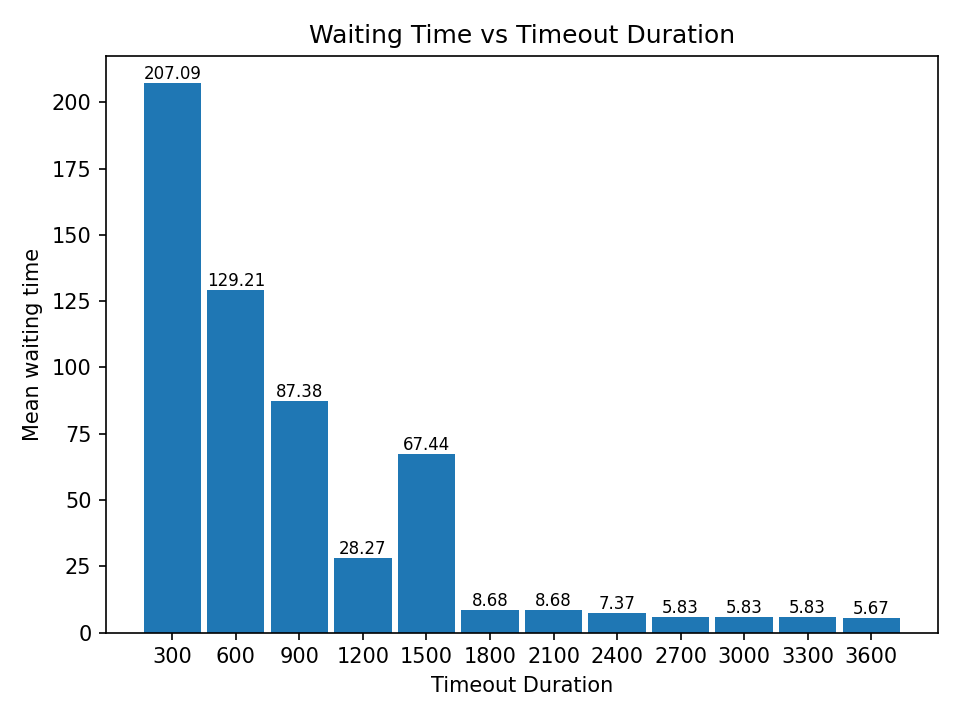
\includegraphics[width=\textwidth]{results/easy_balanced_run/plots/waiting_time_bar.png}\\[0.5\baselineskip]
  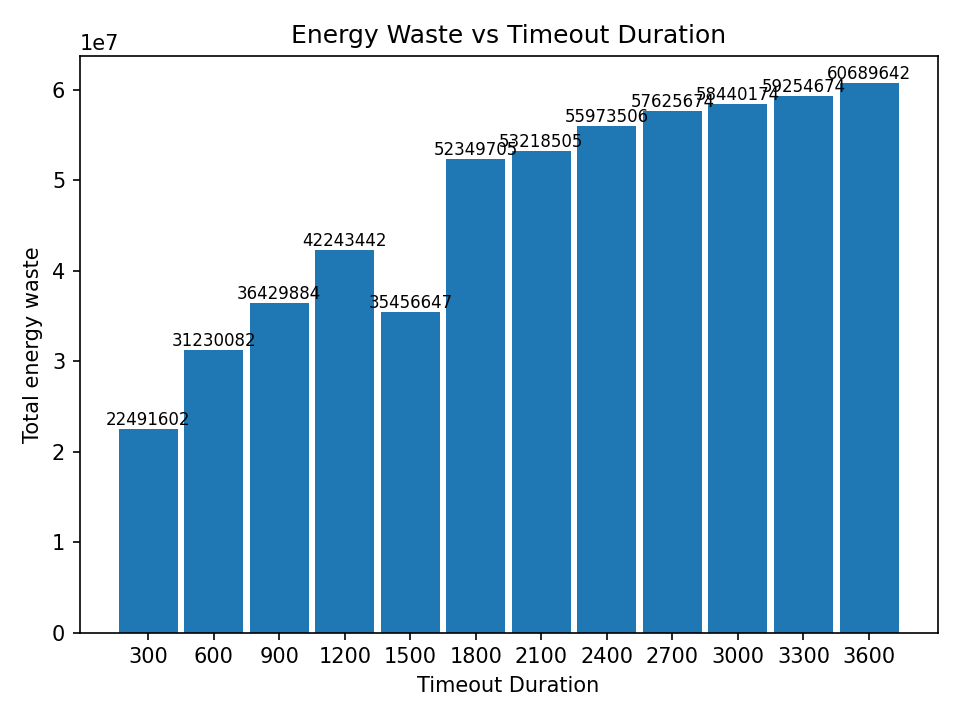
\includegraphics[width=\textwidth]{results/easy_balanced_run/plots/energy_waste_bar.png}
  \caption{EASYBalanced sweep across timeout values. Plots generated with \texttt{plot\_metrics.ipynb}.}
  \label{fig:balanced-plots}
\end{figure}

\subsection{EASYAdaptive}
Figure~\ref{fig:adaptive-plots} shows that adaptive thresholds cut waiting time dramatically at short timeouts: the mean drops from \SI{207}{\second} to \SI{56.6}{\second} at \SI{300}{\second}. The price is higher energy waste because more sleepers are woken proactively, especially when queue pressure is high. As the timeout increases, the advantage in waiting time narrows but energy continues to climb, indicating diminishing returns for aggressive waking beyond \SI{1500}{\second}.

\begin{figure}[h]
  \centering
  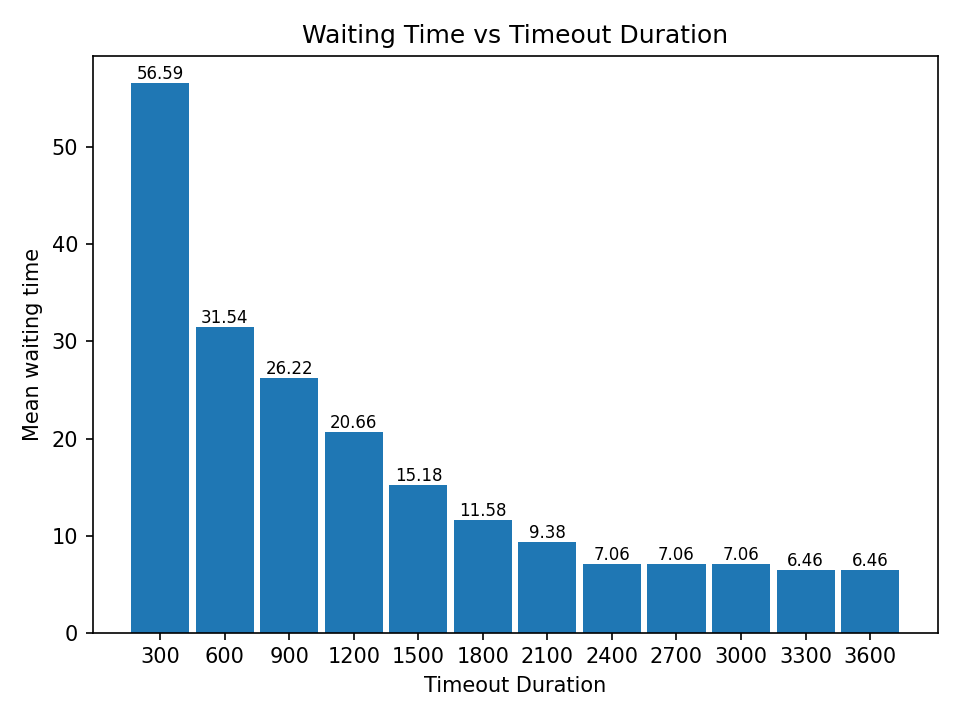
\includegraphics[width=\textwidth]{results/easy_adaptive_run/plots/waiting_time_bar.png}\\[0.5\baselineskip]
  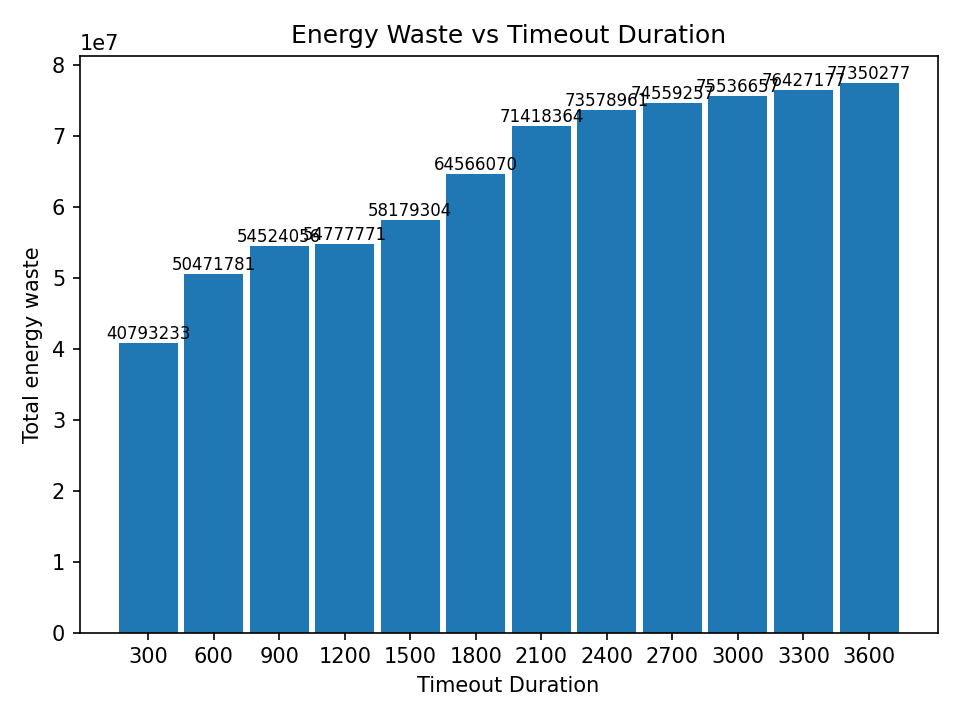
\includegraphics[width=\textwidth]{results/easy_adaptive_run/plots/energy_waste_bar.png}
  \caption{EASYAdaptive sweep across timeout values.}
  \label{fig:adaptive-plots}
\end{figure}

\subsection{Comparative Summary}
Table~\ref{tab:comparison} contrasts the two heuristics. Waiting times are reported in seconds; energy waste is normalised in \si{\mega\joule} to ease comparison. EASYAdaptive dominates latency for all timeouts, but the energy budget grows by roughly \SIrange{18}{24}{\mega\joule} at the short end and more than \SI{16}{\mega\joule} near \SI{3600}{\second}. Operators can therefore select the heuristic that best fits their waiting-time vs.\ energy target.

\begin{table}[h]
  \centering
  \caption{Mean waiting time and total energy waste for each timeout. Energy values are in \si{\mega\joule}.}
  \label{tab:comparison}
  \begin{tabular}{@{}rrrrr@{}}
    \toprule
    Timeout (s) & $\bar{W}$ Balanced & $E_{\mathrm{waste}}$ Balanced & $\bar{W}$ Adaptive & $E_{\mathrm{waste}}$ Adaptive \\
    \midrule
    300 & 207.1 & 22.49 & 56.6 & 40.79 \\
    600 & 129.2 & 31.23 & 31.5 & 50.47 \\
    900 & 87.4 & 36.43 & 26.2 & 54.52 \\
    1200 & 28.3 & 42.24 & 20.7 & 54.78 \\
    1500 & 67.4 & 35.46 & 15.2 & 58.18 \\
    1800 & 8.7 & 52.35 & 11.6 & 64.57 \\
    2100 & 8.7 & 53.22 & 9.4 & 71.42 \\
    2400 & 7.4 & 55.97 & 7.1 & 73.58 \\
    2700 & 5.8 & 57.63 & 7.1 & 74.56 \\
    3000 & 5.8 & 58.44 & 7.1 & 75.54 \\
    3300 & 5.8 & 59.25 & 6.5 & 76.43 \\
    3600 & 5.7 & 60.69 & 6.5 & 77.35 \\
    \bottomrule
  \end{tabular}
\end{table}

\section{Discussion}
\paragraph{When to deploy EASYBalanced.} Use this mode if energy conservation is the primary objective and you can tolerate elevated waiting time when nodes cycle aggressively. Once the timeout is set high enough to keep machines warm, waiting time aligns with adaptive modes while energy remains significantly lower.

\paragraph{When to deploy EASYAdaptive.} This mode is preferable when service-level objectives emphasise latency, especially for short timeout configurations or bursty arrivals. The energy premium is predictable and can be bounded tighter by tuning the heuristic constants (\texttt{SMALL\_SHORTFALL}, \texttt{QUEUE\_DEC}, etc.).

\section{Reproduction Notes}
\begin{itemize}
  \item Plots: rerun \texttt{plot\_metrics.ipynb} with \texttt{results\_dir} set to the desired sweep folder to refresh figures after any new simulation runs.
  \item Gantt charts: \texttt{create\_ganttchart.ipynb} reads per-timeout \texttt{node\_log.csv} to visualise utilisation for specific runs.
  \item Raw metrics: CSV summaries for each algorithm reside alongside the plots (\texttt{summary.csv}) and capture the statistics tabulated above.
\end{itemize}

\begin{thebibliography}{1}
\bibitem{easy}
Feitelson, Dror G. ``Scheduling Parallel Jobs.'' In \emph{Job Scheduling Strategies for Parallel Processing}, Springer, 1995.
\end{thebibliography}

\end{document}
